\documentclass[11pt]{article}
\usepackage{fullpage}
\usepackage[cm-default]{fontspec}
\usepackage{xgreek}
\usepackage{float}
\usepackage{xunicode}
\usepackage{xltxtra}
\usepackage{algorithm}
\usepackage{algpseudocode}
\usepackage{amsmath}
\usepackage{mathtools}
\usepackage{unicode-math}
\usepackage{fontspec}
\usepackage{caption}
\usepackage{subcaption}
\usepackage{soul}
\usepackage[colorlinks,urlcolor=blue]{hyperref}

\setmainfont{CMU Serif}

\title{Ανάπτυξη Λογισμικού για Πληροφοριακά Συστήματα}
\author{Παναγιώτης Φωτόπουλος\\
  \texttt{sdi1300195@di.uoa.gr}
  \and Μάνος Πιτσικάλης\\
  \texttt{sdi1300143@di.uoa.gr}}
\date{Χειμερινό εξάμηνο ακαδημαϊκού έτους 2016-2017}

\begin{document}

\maketitle


\section{Εισαγωγή - Γενικά}
Η παρούσα εργασία αποτελεί υλοποίηση μιας λύσης για το πρόβλημα του ελάχιστου μονοπατιού σε γράφους. Μετά από μια πρώτη απλή προσέγγιση με αμφίδρομη αναζήτηση στο γράφο προστέθηκαν ειδικές δομές για απάντηση ερωτημάτων, καθώς και πολυνηματισμός για την παράλληλη επεξεργασία τους, όπως περιγράφονται στις επιμέρους εκφωνήσεις.\\\\
\textbf{\underline{Μεταγλώττιση \& Εκτέλεση:}}
\begin{itemize}
\item Για το τελικό εκτελέσιμο:\\
> make spath\\
> ./spath <initial graph file> <workload file>\\
Σημείωση: αν η main μεταγλωττισθεί με δήλωση VERBOSE\_MODE, δηλαδή εκτελεστεί η εντολή: \\
> gcc -c -Wall -Ofast sources/mains\_and\_utilities/main.c -DVERBOSE\_MODE -o objects/main.o\\
(πριν την εντολή make), τότε κατά την εκτέλεση του workload εμφανίζεται το ποσοστό του workload που έχει εκτελεστεί. Αυτό μπορεί να φανεί χρήσιμο κατά την εκτέλεση πολύ μεγάλων workloads όπου η εκτέλεση παίρνει πολλή ώρα.
\item Για το εκτελέσιμο του 2ου part (χωρίς πολυνηματισμό):\\
> make part2\_spath\\
> ./part2\_spath <initial graph file> <workload file>
\item Για το unit testing:\\
> make unittesting\\
> ./unittesting
\end{itemize}

\section{Λεπτομέρειες υλοποίησης Part 1}
\begin{itemize}
\item \textbf{Δομές αποθήκευσης}\\ Για την αποθήκευση του γράφου χρησιμοποιούνται δύο ευρετήρια (index-buffer): ένα για τις εξερχόμενες ακμές και ένα για τις εισερχόμενες ακμές. Στις αναζητήσεις και γενικά όπου χρειάζονται λίστες, για την αποφυγή πολλών malloc χρησιμοποιούνται λίστες υλοποιημένες με πίνακα, οι οποίες και επαναχρησιμοποιούνται όταν χρειαστεί. Δηλάδη γινέται μια φορά malloc, αν χρειαστεί γίνεται realloc, και με την λήξη της εκτέλεσης γίνεται η αποδέσμευση της μνήμης. Επιπλέον, στις αναζητήσεις και όπου αλλού χρειάζεται δομή για να σημαδεύονται οι κόμβοι (π.χ.στην bidirectional-bfs η δομή visited) χρησιμοποιείται πίνακας A ίσος με τον αριθμό των στοιχείων με versioning, δηλαδή αν το στοιχείο x έχει επισκεφτεί οταν γίνεται αναζήτηση με version v τότε A[x]=v, αν κάποιο στοιχείο y δεν έχει επισκεφτεί τότε θα ισχύει A[y]<v, έτσι η αρχικοποιήση γίνεται μόνο μία φορά και ο έλεγχος γίνεται σε O(1).
\item \textbf{Αναζήτηση}\\ Για την αναζήτηση χρησιμοποιήθηκε η bidirectional Breadth-First Search, όπως περιγράφεται στην εκφώνηση, με τις εξής λεπτομέρειες/βελτιώσεις:
\begin{itemize}
\item Στην αρχή της κάθε επανάληψης, θα επιλεχθεί για επέκταση η BFS η οποία έχει την χαμηλότερη τιμή στην εξής ευρετική:\\
\textit{<αριθμός "παιδιών" προς επέκταση> + <αριθμός "εγγονιών" προς επέκταση (σε επόμενη επανάληψη)>}\\
Με αυτόν τον τρόπο, αποφεύγεται η σπατάλη χρόνου σε καταστάσεις όπου από τη μία κατεύθυνση υπάρχουν πάρα πολλά πιθανά μονοπάτια, ενώ από την άλλη λίγα ή μόνο ένα.
\item Η αναζήτηση γίνεται ανά "επίπεδα": Σε κάθε επανάληψη, η τρέχουσα BFS επισκέπτεται \textbf{\underline{όλα}} τα παιδιά του τρέχοντος βάθους.
\end{itemize}
\item \textbf{Unit testing}\\ Έχει υλοποιηθεί unit testing στις βασικές δομές με χρήση check. Για την σώστη λειτουργία του είναι απαραίτητο να υπάρχει εγκατεστημένο το {\color{blue}\underline{\href{https://libcheck.github.io/check/}{Check}}}.
\item \textbf{Εισαγωγή ακμών}\\ Κατά την εισαγωγή ακμών, ο έλεγχος ύπαρξης ακμής γίνεται στον κόμβο με τις λιγότερες ακμές στην αντίστοιχη κατεύθυνση (εισερχόμενες-εξερχόμενες) για εξοικονόμηση χρόνου. Δοκιμάστηκε η χρήση hashtable για να γίνεται σε O(1) ο έλεγχος αυτός, αλλά αυτή η προσέγγιση αποδείχθηκε μη αποδοτική καθώς επηρέαζε σημαντικά τη χρήση μνήμης, καθώς και τον συνολικό χρόνο (ενημέρωση του hashtable). Σημείωση: υπάρχουν τα αρχεία για το hash table (hash.c, hash.h), αλλά δεν χρησιμοποιούνται στο τελικό πρόγραμμα.
\end{itemize}
\section{Λεπτομέρειες υλοποίησης Part 2}
\begin{itemize}
\item \textbf{StonglyConnectedComponents}\\
Για την εύρεση των SCCs χρησιμοποιήθηκε ο αλγόριθμος του Tarjan, αλλά τροποποιημένος ώστε αντί αναδρομικά να τρέχει επαναληπτικά. Αυτή η αλλαγή επέτρεψε την επεξεργασία μεγαλύτερων workloads, στα οποία στην αναδρομική προσέγγιση "έσκαγε" η στοίβα.
\item \textbf{Grail Index}\\
Και εδώ τροποποιήθηκε η αρχική αναδρομική υλοποίηση σε επαναληπτική. Επίσης, ο αριθμός των labels που επιλέχθηκε (πειραματικά, μετά από διάφορες δοκιμές) είναι 5.
\item \textbf{(Weakly) Connected Components Index}\\
Για την αρχική εύρεση των CC χρησιμοποιήθηκε Depth-First-Search. Η αποθήκευση τους γίνεται σε έναν πίνακα με μέγεθος ίσο με το πλήθος των κόμβων, και όταν γίνει ένωση μεταξύ δύο components χρησιμοποιείται η δομή Updated, η οποία υλοποιήθηκε και δοκιμάστηκε με τους εξής τρόπους:
\begin{itemize}
\item H πρώτη υλοποιήση έγινε με την δομή της εκφώνησης η οποία φάνηκε να είναι η χειρότερη σε σχέση με τις άλλες δύο που δοκιμάστηκαν.
\item Η δεύτερη υλοποιήση χρησιμοποιούσε ένα πίνακα με δείκτες σε λίστες (τις οποίες παίρνει απο μία δομη με επαναχρησιμοποιήσιμες λιστες (list pool)) με τα συνδεδεμένα components του κάθε cc. Ωστόσο αυτή η λύση απαίτουσε rebuild. Σε κάθε rebuild ενημερώνεται το ευρετήριο και "αδειάζονται" οι λίστες του updated. Κι αυτή η υλοποίηση όμως φάνηκε να μην είναι η καλύτερη απο αυτές που δοκιμάστηκαν.
\item Η τρίτη και αυτή που επιλέξαμε για τον πίνακα updated χρησιμοποιεί disjoint sets με χρήση union by rank και path compression. Περισσότερες πληροφορίες βρίσκονται εδώ: {\color{blue}\underline{\href{https://en.wikipedia.org/wiki/Disjoint-set\_data\_structure\#Union\_by\_rank}{Disjoint Sets (Wikipedia)}}}. Σε αυτή την υλοποιήση κρίναμε πως το rebuild στο update index δεν είναι απαραίτητο καθώς καλυπτεί αυτή την ανάγκη σε μεγάλο βαθμό το path compression.
\end{itemize}
\end{itemize}
\section{Λεπτομέρειες υλοποίησης Part 3}
\begin{itemize}
\item \textbf{JobScheduler}\\
Ο JobScheduler υλοποιήθηκε όπως ζητείται στην εκφώνηση. Ο τερματισμός των threads γίνεται με αποστολή queries με ειδικό version 0.
\item \textbf{Πολυνηματισμός}\\
Έγιναν αλλαγές στον κώδικα των προηγούμενων parts, ώστε να είναι συμβατός με πολυνηματισμό. Σε αυτές περιλαμβάνονται: error handling \& printing, το σύστημα versioning για την σωστή εκτέλεση των ερωτημάτων στους δυναμικούς γράφους, όπως επίσης το ότι οι ουρές και οι δομές για μαρκάρισμα στις αναζητήσεις (και γενικά όπου ήταν απαραίτητο) μεταφέρθηκαν στα threads αντί να είναι μέλος του γράφου.
\item \textbf{Connected Components Disjoint Sets}\\
Καθώς κάθε ερώτημα έχει δικό του version, είναι απαραίτητη η διατήρηση των πληροφορίων όπως η ενώση μεταξυ CC, για κάθε version, στο πίνακα ευρετηρίου των CC και την δομη updated. Γι αυτό και στο updated για κάθε ενημέρωση οι πληροφορίες του κάθε CC (parent,rank,version) διατηρούνται σε λίστες στον πίνακα updated (οι οποίες δίνονται από το list pool). Για εξοικονόμηση μνήμης, αλλά και επείδη το path compression δεν είναι δυνάτο σε πλήρη βαθμό λόγω πολυνηματισμού, γίνεται rebuild στο τέλος κάθε ριπής με χρήση path compression. Έτσι ενημερώνεται ο βασικός πίνακας, και στην συνέχεια γίνεται το "άδειασμα" των λιστών καθιστώντας τες διαθέσιμες για μελλοντική χρήση σε άλλα CC, μειώνοντας έτσι την ανάγκη μνήμης. 

\end{itemize}
\section{Μετρήσεις}
Oι μετρήσεις έγιναν σε laptop με επεξεργαστή i7-3612QM (2.10 GHz, 4 cores, 8 threads) και μνήμη DDR3 1600MHz 8 GB. Για την μέτρηση των χρόνων χρησιμοποιήθηκε η συνάρτηση time και για την μέτρηση της απαιτούμενης χρησιμοποιούμε την τιμή (VmPeak) της τρέχουσας διεργασίας (\textit{cat /proc/pid\_of\_spath/status |grep VmPeak}).
\begin{enumerate}
\item Παρακάτω ακολουθεί σύγκριση στους χρόνους και στην απαιτούμενη μνήμη για κάθε μέρος της εργασίας με εισόδους τα δυναμικά και τα στατικά datasets που δόθηκαν.\\
\begin{table}[H]
\caption{Dynamic Datasets times}

\begin{minipage}{.5\textwidth}
\footnotesize
\label{ddt}
\tabcolsep=0.11cm
\begin{tabular}{|l|l|l|l|}
\hline
\multicolumn{4}{|l|}{Dynamic Datasets times (MM:SS.000)} \\ \hline
          & Part 1      & Part 2     & Part 3-8 threads  \\ \hline
Tiny      & 00:00.001   & 00:00.002  & 00:00.004         \\ \hline
Small     & 00:00.453   & 00:00.519  & 00:00.596         \\ \hline
Medium    & 00:01.539   & 00:01.760  & 00:02.530         \\ \hline
Large     & 11:01.551   & 10:28.650  & 03:41.225         \\ \hline
Large 2   & 50:29.401   & 47:21.940  & 17:35.641         \\ \hline
\end{tabular}
\end{minipage}%
\begin{minipage}{.5\textwidth}
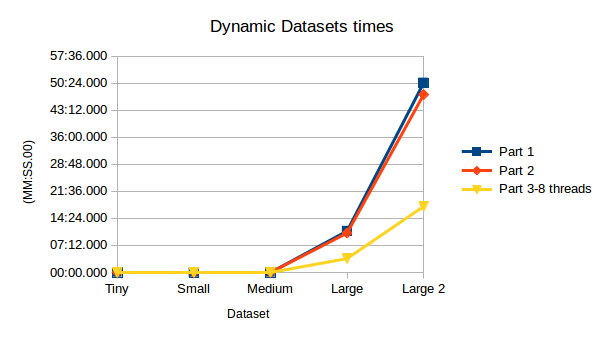
\includegraphics[scale=0.5]{DynamicDatasets_times.png}
\end{minipage}%
\end{table}

\begin{table}[H]
\caption{Dynamic Datasets Memory Usage}
\begin{minipage}{.5\textwidth}
\centering
\footnotesize
\tabcolsep=0.11cm
\label{ddm}
\begin{tabular}{|l|l|l|l|}
\hline
\multicolumn{4}{|l|}{Dynamic Dataset VmPeak (KB)} \\ \hline
         & Part 1 Vm & Part 2  & Part 3-8 threads \\ \hline
Large    & 1414896   & 1458116 & 2414616          \\ \hline
Large 2  & 1829748   & 2335964 & 3291848          \\ \hline
\end{tabular}
\end{minipage}%
\begin{minipage}{.5\textwidth}
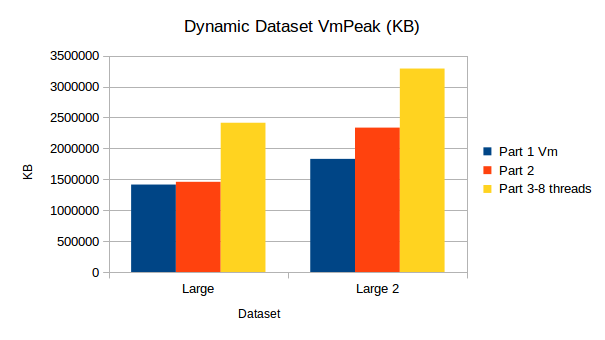
\includegraphics[scale=0.5]{DynamicDatasets_VmPeak.png}
\end{minipage}%
\end{table}

\begin{table}[H]
\caption{Static Datasets times}
\begin{minipage}{.5\textwidth}
\centering
\footnotesize
\tabcolsep=0.11cm
\label{sdt}
\begin{tabular}{|l|l|l|l|}
\hline
\multicolumn{4}{|l|}{Static Datasets times (MM:SS.000)} \\ \hline
        & Part 1         & Part 2    & Part 3-8 threads \\ \hline
Medium  & 00:01.434      & 00:02.538 & 00:02.637        \\ \hline
Large   & 05:03.604      & 01:54.640 & 00:51.800        \\ \hline
Large 2 & \textgreater3H & 26:28.035 & 08:31.369        \\ \hline
\end{tabular}
\end{minipage}%
\begin{minipage}{.5\textwidth}
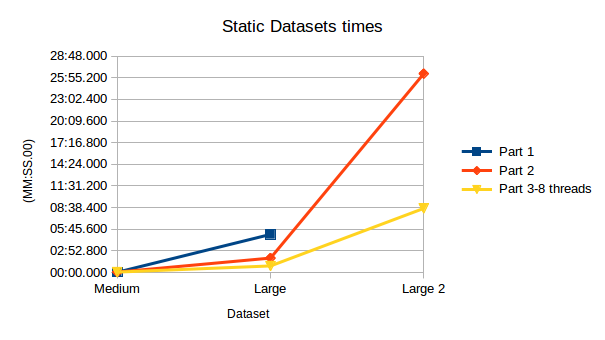
\includegraphics[scale=0.5]{StaticDatasets_times.png}
\end{minipage}%
\end{table}

\begin{table}[H]
\caption{Static Datasets Memory Usage}
\begin{minipage}{.5\textwidth}
\centering
\footnotesize
\tabcolsep=0.11cm
\label{sdm}
\begin{tabular}{|l|l|l|l|}
\hline
\multicolumn{4}{|l|}{Static Datasets times (MM:SS.000)} \\ \hline
        & Part 1         & Part 2    & Part 3-8 threads \\ \hline
Medium  & 00:01.434      & 00:02.538 & 00:02.637        \\ \hline
Large   & 05:03.604      & 01:54.640 & 00:51.800        \\ \hline
Large 2 & \textgreater3H & 26:28.035 & 08:31.369        \\ \hline
\end{tabular}
\end{minipage}%
\begin{minipage}{.5\textwidth}
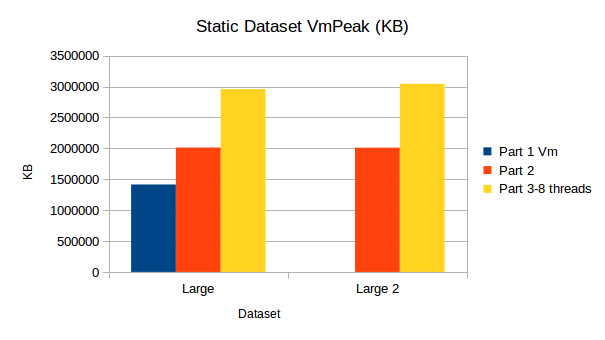
\includegraphics[scale=0.5]{StaticDatasets_VmPeak.png}
\end{minipage}%
\end{table}

\item Aκολουθεί σύγκριση των χρόνων και της απαιτούμενης μνήμης στο τελευταίο κομμάτι της εργασίας με παράμετρο τον αριθμό των νημάτων για δυναμικά και στατικά datasets.\\
\begin{table}[H]
\caption{Dynamic Dataset Multithreading times}
\begin{minipage}{.5\textwidth}
\centering
\footnotesize
\tabcolsep=0.11cm
\label{ddmt}
\scalebox{0.9}{
\begin{tabular}{|l|l|l|l|l|}
\hline
\multicolumn{5}{|l|}{Dynamic Dataset Multithreading times (MM:SS.000)} \\ \hline
Threads    & N=2          & N=4          & N=8          & N=16         \\ \hline
Large      & 05:57.266    & 04:03.300    & 03:41.225    & 03:42.664    \\ \hline
Large 2    & 26:30.534    & 18:45.376    & 17:35.641    & 17:57.566    \\ \hline
\end{tabular}}
\end{minipage}%
\begin{minipage}{.5\textwidth}
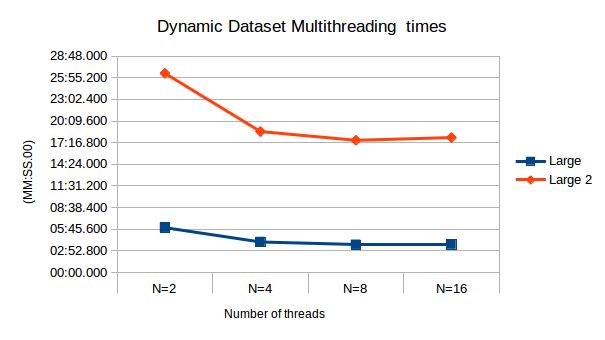
\includegraphics[scale=0.5]{DynamicDatasetMultithreading_times.png}
\end{minipage}%
\end{table}

\begin{table}[H]
\caption{Dynamic Dataset Multithreading Memory Usage}
\begin{minipage}{.5\textwidth}
\centering
\footnotesize
\tabcolsep=0.11cm
\label{ddmm}
\scalebox{0.9}{
\begin{tabular}{|l|l|l|l|l|}
\hline
\multicolumn{5}{|l|}{Dynamic Dataset Multithreading VmPeak(KB)} \\ \hline
Threads     & N=2        & N=4        & N=8        & N=16       \\ \hline
Large       & 1677284    & 1923060    & 2414616    & 3397252    \\ \hline
Large 2     & 2579536    & 2825312    & 3291848    & 4299972    \\ \hline
\end{tabular}
}
\end{minipage}%
\begin{minipage}{.5\textwidth}
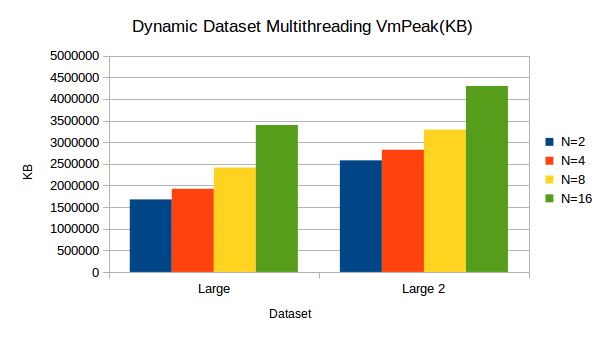
\includegraphics[scale=0.5]{DynamicDatasetMultithreading_VmPeak.png}\\
\end{minipage}%
\end{table}

\begin{table}[H]
\caption{Static Dataset Multithreading times}
\begin{minipage}{.5\textwidth}
\centering
\footnotesize
\tabcolsep=0.11cm
\label{sdmt}
\scalebox{0.9}{
\begin{tabular}{|l|l|l|l|l|}
\hline
\multicolumn{5}{|l|}{Static Dataset Multithreading times (MM:SS.000)} \\ \hline
Threads    & N=2          & N=4          & N=8          & N=16        \\ \hline
Large      & 01:53.454    & 01:18.555    & 01:01.018    & 00:51.800   \\ \hline
Large 2    & 16:54.585    & 10:05.976    & 08:30.127    & 08:31.690   \\ \hline
\end{tabular}
}
\end{minipage}%
\begin{minipage}{.5\textwidth}
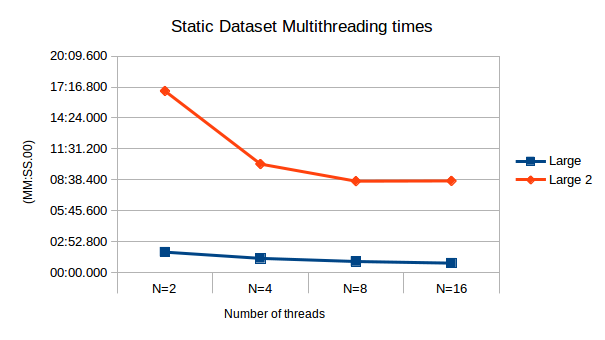
\includegraphics[scale=0.5]{DynamicStaticMultithreading_times.png}
\end{minipage}%
\end{table}

\begin{table}[H]
\caption{Static Dataset Multithreading Memory Usage}
\begin{minipage}{.5\textwidth}
\centering
\footnotesize
\tabcolsep=0.11cm
\label{sdmmu}
\scalebox{0.9}{
\begin{tabular}{|l|l|l|l|l|}
\hline
\multicolumn{5}{|l|}{Static Dataset Multithreading VmPeak(KB)} \\ \hline
Threads    & N=2        & N=4        & N=8        & N=16       \\ \hline
Large      & 2222564    & 2468340    & 2959892    & 3943000    \\ \hline
Large 2    & 2307580    & 2553356    & 3044908    & 3950336    \\ \hline
\end{tabular}
}
\end{minipage}%
\begin{minipage}{.5\textwidth}
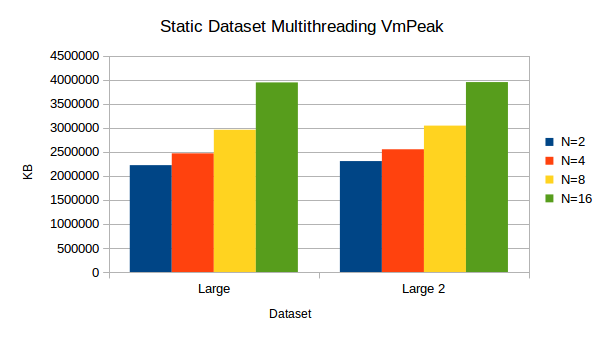
\includegraphics[scale=0.5]{DynamicStaticMultithreading_VmPeak.png}
\end{minipage}%
\end{table}
\end{enumerate}
\end{document}
